\chapter{Concurrent ABS}
In an ideal world, we would like to solve all our problems using parallelism but unfortunately, it can't be applied to all parallel problems and ABS is no exception. As soon as there are data-dependencies, like we have them in the Sugarscape model in the form of the read/write environment and synchronous agent-interactions, and to a lesser extent in the monadic SIR with the Rand monad, we cannot avoid concurrency. More general, this is due to the fact that agents are executed within a monadic context, from which the  sequencing of effectful computations immediately follows - the very meaning of the Monad abstraction. Indeed, we have shown both by argument and measurement in the previous chapter the very fact that parallelism is simply not applicable to monadic execution of agents due to sequencing of effects, which renders all attempts of running monadic agents in parallel void. In this chapter we discuss the use of concurrency to run agents which have a monadic context in parallel - which is the only way we can execute monadic agents at the same time.

\medskip

Traditional approaches to concurrency follow a lock-based approach, where sections which access shared data are synchronised through synchronisation primitives like mutexes, semaphores, monitors,... The lock-based path is a well trodden one, with all problems and benefits well established. In this chapter we follow a different path and look into using Software Transactional Memory (STM) for implementing concurrent ABS, which promises to overcome the problems of lock-based approaches. Although STM exists in other languages as well, Haskell was one of the first to natively build it into its core, thus it is a natural choice to follow that direction when already investigating pure functional ABS.

Unfortunately, as soon as we employ concurrency, we lose all static guarantees about reproducibility and the use of STM is no exception. Still, STM has the unique benefit that it can guarantee the lack of persistent side-effects at compile time, allowing unproblematic retries of transactions, something of fundamental importance in STM as will be described below. This implies also another \textit{very} compelling advantage of STM over unrestricted lock-based approaches: by using STM, we can reduce the side-effects allowed substantially and guarantee at compile time, that the differences between runs of same initial conditions will only stem from the fact that we run the simulation concurrently - \textit{and from nothing else}. All this makes the use of STM very compelling and to our best knowledge we are the very first to investigate the use of STM for implementing concurrent ABS in a systematic way.

\medskip

The paper \cite{discolo_lock_2006} gives a good indication how difficult and complex constructing a correct concurrent program is and shows how much easier, concise and less error-prone an STM implementation is over traditional locking with mutexes and semaphores. More important, it shows that STM consistently outperforms the lock-based implementations. We follow this work and compare the performance of lock-based and STM implementations and hypothesise that the reduced complexity and increased performance will be directly applicable to ABS as well.

We present two case studies using the already introduced SIR (Chapter \ref{sec:sir_model}) and Sugarscape (Chapter \ref{sec:sugarscape}) models. We compare the performance of lock-based and STM implementations in each case where we investigate both the scaling performance under increasing number of CPUs and agents. We show that the STM implementations consistently outperform the lock-based ones and scale much better to increasing number of CPUs both on local machines and on Amazon Cloud Services.

Note that there exists also the actor model of concurrency, which is especially well suited to implement concurrent applications in functional languages. We give a short overview over it, existing research and its use in ABS in the section \ref{sec:actors} but leave it for further research as it has very different implications, which are beyond the focus of this thesis.

TODO: shortening, no comparison to io or repast: the story is "concurrency with compile time guarantees", only mention that an io based single lock performs much worse in sir and slightly worse in sugarscape. leave Array i IORef for further research

\section{Software Transactional Memory}
Software Transactional Memory was introduced by \cite{shavit_software_1995} in 1995 as an alternative to lock-based synchronisation in concurrent programming which, in general, is notoriously difficult to get right. This is because reasoning about the interactions of multiple concurrently running threads and low level operational details of synchronisation primitives is \textit{very hard}. The main problems are \cite{marlow_parallel_2013}:

\begin{itemize}
	\item Race conditions due to forgotten locks;
	\item Deadlocks resulting from inconsistent lock ordering;
	\item Corruption caused by uncaught exceptions;
	\item Lost wake-ups induced by omitted notifications.
\end{itemize}

What is worse, concurrency does not compose. It is very difficult to write two functions (or methods in an object) acting on concurrent data which can be composed into a larger concurrent behaviour. The reason for the difficulty is that one has to know about the internal details of locking, which breaks encapsulation and makes composition dependent on knowledge about their implementation. Therefore, it is impossible to compose two functions where, for example, one withdraws some amount of money from an account and the other deposits this amount of money into a different account. The problem is that one ends up with a temporary state where the money is in neither of the accounts, creating an inconsistency and a potential source for errors because threads can be rescheduled at any time.

STM promises to solve all of these problems for a low cost by executing actions \textit{atomically}, where modifications made in such an action are invisible to other threads and changes by other threads are also invisible until actions are committed - STM actions are atomic and isolated. When an STM action exits, either one of two outcomes happen: if no other thread has modified the same data as the thread running the STM action, then the modifications performed by the action will be committed and become visible to the other threads. If other threads have modified the data then the modifications will be discarded, the action rolled back and automatically restarted.

\subsection{Software Transactional Memory in Haskell}
The work of \cite{harris_composable_2005, harris_transactional_2006} added STM to Haskell, which was one of the first programming languages to incorporate STM with composable operations into its main core. In the Haskell implementation, STM actions run within the \texttt{STM} Monad. This restricts the operations to only STM primitives as shown below. This means that \texttt{STM} actions are always repeatable without persistent side effects because such persistent side effects (for example writing to a file, launching a missile) are not possible in the \texttt{STM} Monad. This is also the fundamental difference to \texttt{IO}, where all bets are off and \textit{everything} is possible because \texttt{IO} can run everything without restrictions.

Thus, the ability to \textit{restart} an action without any persistent effects is only possible due to the nature of Haskell's type system and by restricting the effects to \texttt{STM} only, ensures that only controlled effects, which can be rolled back, occur.

STM comes with a number of primitives to share transactional data. Amongst others the most important ones are:

\begin{itemize}
	\item \texttt{TVar} - a transactional variable which can be read and written arbitrarily;
	
	\item \texttt{TMVar} - a transactional \textit{synchronising} variable which is either empty or full. To read from an empty or write to a full \texttt{TMVar} will cause the current thread to block and retry its transaction when \textit{any} transactional primitive of this action has changed.
	
	\item \texttt{TArray} - a transactional array where each cell is an individual transactional variable \texttt{TVar}, allowing more finer-grained transactions instead of having the whole array in a \texttt{TVar}.
	
	\item \texttt{TChan} - a transactional channel, representing an unbounded FIFO channel, based on a linked list of \texttt{TVar}.
\end{itemize}

Furthermore STM also provides combinators to deal with blocking and composition:

\begin{itemize}
	\item \texttt{retry :: STM ()} retries an \texttt{STM} action. This will cause to abort the current transaction and block the thread it is running in. When \textit{any} of the transactional data primitives have changed, the action will be run again. This is useful to await the arrival of data in a \texttt{TVar}, or put more general, to block on arbitrary conditions. 
	
	\item \texttt{orElse :: STM a $\rightarrow$ STM a $\rightarrow$ STM a} allows us to combine two blocking actions where either one is executed, but not both. The first action is run and if it is successful its result is returned. If it retries, then the second is run and if that one is successful its result is returned. If the second one retries, the whole \texttt{orElse} retries. This can be used to implement alternatives in blocking conditions, which can obviously be nested arbitrarily.
\end{itemize}

To run an \texttt{STM} action the function \texttt{atomically :: STM a $\rightarrow$ IO a} is provided, which performs a series of \texttt{STM} actions atomically within the \texttt{IO} Monad. It takes the \texttt{STM} action, which returns a value of type \texttt{a} and returns an \texttt{IO} action which returns a value of type \texttt{a}. The \texttt{IO} action then can only be executed from within the \texttt{IO} Monad, either within the main thread or an explicitly forked thread.

STM in Haskell is implemented using optimistic synchronisation, which means that instead of locking access to shared data, each thread keeps a transaction log for each read and write to shared data that it makes. When the transaction exits, the thread checks whether it has a consistent view to the shared data or not. It checks whether other threads have written to memory it has read, thus it can identify whether a rollback is required or not.

However, STM does not come without issues. The authors of \cite{perfumo_limits_2008} analyse several Haskell STM programs with respect to their transactional behaviour. They identified the roll-back rate as one of the key metrics, which determines the scalability of an application. Although STM might promise better performance, they also warn of the overhead it introduces, which could be quite substantial in particular for programs which do not perform much work inside transactions as their commit overhead is high.

\subsection{STM Examples}
We provide two examples to demonstrate the use and semantics of STM. The first example is an implementation of the aforementioned functionality, where money is withdrawn from one account and transferred to another. The implementing function \texttt{transferFunds} takes two \texttt{TVar}, holding the account balances, and the amount to exchange. It executes using \texttt{atomically}, therefore running in the \texttt{IO} Monad. It uses the two functions \texttt{withdraw} and \texttt{deposit} which do the work of withdrawing some amount from one account and depositing some amount to another. This example demonstrates how easily STM can be used: the implementation looks quite straightforward, simply swapping values, without any locking involved or special handling of concurrency, other than the use of \texttt{atomically}.

\begin{HaskellCode}
transferFunds :: TVar Integer -> TVar Integer -> Integer -> IO ()
transferFunds from to n = atomically (do
  withdraw from n
  deposit to n)
  
withdraw :: TVar Integer -> Integer -> STM ()
withdraw account amount = do
  balance <- readTVar account
  writeTVar (balance - amount)
  
deposit :: TVar Integer -> Integer -> STM ()
deposit account amount = do
  balance <- readTVar account
  writeTVar (balance + amount)
\end{HaskellCode}

In the second example we show the retry semantics of STM, by using it within a \texttt{StateT} transformer where \texttt{STM} is the innermost Monad. It is important to understand that \texttt{STM} does not provide a transformer instance for very good reasons. If it would provide a transformer then we could make \texttt{IO} the innermost Monad and perform \texttt{IO} actions within \texttt{STM}. This would violate the retry semantics, as in case of a retry, \texttt{STM} is unable to undo the effects of \texttt{IO} actions in general. This stems from the fact that the \texttt{IO} type is simply too powerful and we cannot distinguish between different kinds of \texttt{IO} actions in the type, be it simply reading from a file or actually launching a missile. Let's look at the example code:

\begin{HaskellCode}
stmAction :: TVar Int -> StateT Int STM Int 
stmAction v = do
  -- print a debug output and increment the value in StateT 
  Debug.trace "increment!" (modify (+1))
  -- read from the TVar
  n <- lift (readTVar v)
  -- await a condition: content of the TVar >= 42
  if n < 42
    -- condition not met: retry
    then lift retry
    -- condition met: return content ot TVar
    else return n
\end{HaskellCode}

In this example, the \texttt{STM} is the innermost Monad in a stack with a \texttt{StateT} transformer. When \texttt{stmAction} is run, it prints an \texttt{'increment!'} debug message to the console and increments the value in the \texttt{StateT} transformer. Then it awaits a condition. For as long as \texttt{TVar} is less then 42 the action will retry whenever it is run. If the condition is met, it will return the content of the \texttt{TVar}. We see the combined effects of using the transformer stack where we have both the \texttt{StateT} and the \texttt{STM} effects available. The question is how this code behaves if we actually run it. To do this we need to spawn a thread:

\begin{HaskellCode}
stmThread :: TVar Int -> IO ()
stmThread v = do
  -- the initial state of the StateT transformer
  let s = 0
  -- run the state transformer with initial value of s (0)
  let ret = runStateT (stmAction v) s
  -- atomically run the STM block
  (a, s') <- atomically ret
  -- print final result
  putStrLn("final StateT state     = " ++ show s' ++
           ", STM computation result = " ++ show a)
\end{HaskellCode}

The thread simply runs the \texttt{StateT} transformer layer with the initial value of 0 and then the \texttt{STM} computation through \texttt{atomically} and prints the result to the console. The value of \texttt{a} is the result of \texttt{stmAction} and \texttt{s'} is the final state of the \texttt{StateT} computation. To actually run this example we need the main thread to update the \texttt{TVar} until the condition is met within \texttt{stmAction}:

\begin{HaskellCode}
main :: IO ()
main = do
  -- create a new TVar with initial value of 0
  v <- newTVarIO 0 
  -- start the stmThread and pass the TVar
  forkIO (stmThread v)
  -- do 42 times...
  forM_ [1..42] (\i -> do
    -- use delay to 'make sure' that a retry is happening for ever increment
    threadDelay 10000
    -- write new value to TVar using atomically
    atomically (writeTVar v i))
\end{HaskellCode}

If we run this program, we will see \texttt{'increment!'} printed 43 times, followed by \texttt{'final StateT state = 1, STM computation result = 42'}. This clearly demonstrates the retry semantics where \texttt{stmAction} is retried 42 times and thus prints \texttt{'increment!'} 43 times to the console. The \texttt{StateT} computation, however, is carried out only once and is always rolled back when a retry is happening. The rollback is easily possible in pure functional programming due to persistent data structure, by simply throwing away the new value and retrying with the original value. This example also demonstrates that any \texttt{IO} actions which happen within an \texttt{STM} action are persistent and can obviously not be rolled back. \texttt{Debug.trace} is an \texttt{IO} action masked as pure using \texttt{unsafePerformIO}.

\section{Software Transactional Memory in ABS}
\label{sec:stm_abs}
In this section we give a short overview of how we apply STM to pure functional ABS. In both case studies we fundamentally follow a time-driven, parallel approach as introduced in Chapter \ref{sub:par_strategy}, where the simulation is advanced by a given $\Delta t$ and in each step all agents are executed. To employ parallelism, each agent runs within its own thread and agents are executed in lock-step, synchronising between each $\Delta t$, which is controlled by the main thread. See Figure \ref{fig:stm_abs_structure} for a visualisation of the concurrent, parallel time-driven lock-step approach.

By running each agent in a thread will guarantee the execution in parallel even if the agent has a monadic context. This forces us to evaluate each agents monadic context separately instead of running them all in a common context. This means that we are ending up in the \texttt{IO} Monad because \texttt{STM} can be only transacted from within an \texttt{IO} context due to non-deterministic side effects. This is no contradiction to our original claim. Yes we are running in \texttt{IO} but not the agent behaviour itself, which is a fundamental difference.

An agent thread will block until the main thread sends the next $\Delta t$ and runs the \texttt{STM} action atomically with the given $\Delta t$. When the \texttt{STM} action has been committed, the thread will send the output of the agent action to the main thread to signal it has finished. The main thread awaits the results of all agents to collect them for output of the current step, for example visualisation or writing to a file.

As will be described in subsequent sections, central to both case studies is an environment which is shared between the agents using a \texttt{TVar} or \texttt{TArray} primitive, through which the agents communicate concurrently with each other. To get the environment in each step for visualisation purposes, the main thread can access the \texttt{TVar} and \texttt{TArray} as well. 

\begin{figure}
	\centering
	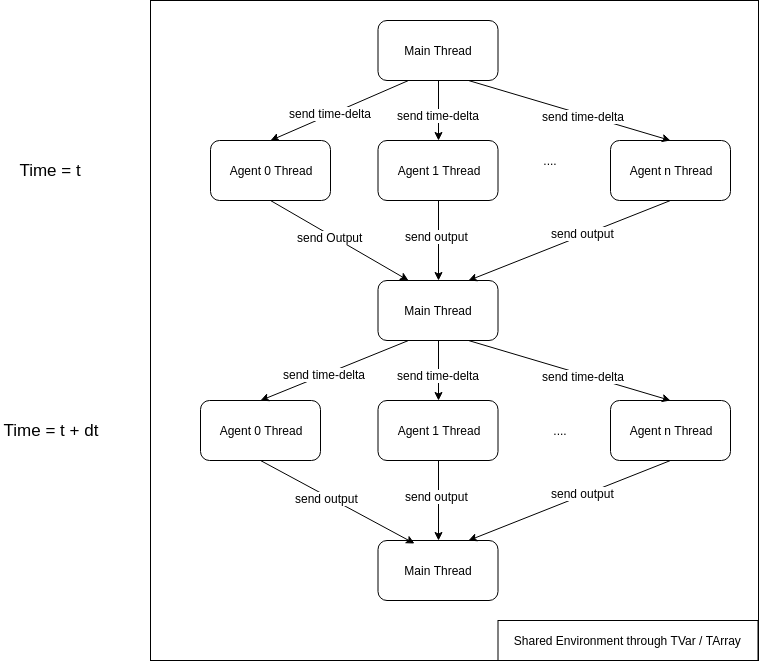
\includegraphics[width=0.7\textwidth, angle=0]{./fig/concurrentabs/stm_abs.png}
	\caption[Diagram of the parallel time-driven lock-step approach]{Diagram of the parallel time-driven lock-step approach.}
	\label{fig:stm_abs_structure}
\end{figure}

\subsection{Adding STM to agents}
We briefly discuss how to add STM to agents on a technical level and also show how to run them within their own threads. We use the SIR implementation as example - applying it to the Sugarscape implementation works exactly the same way and is left as a trivial exercise to the reader.

The first step is to simply add the \texttt{STM} Monad as the innermost level to the already the existing Transformer stack. Further, the environment is now passed as a transactional data primitive to the agent at \textit{construction time}. Thus, the agent does not receive the \texttt{SIREnv} as input any more but receives it through currying when constructing its initial \texttt{MSF}. Further, the agent modifies the \texttt{SIREnv} directly through the \texttt{TVar}, as demonstrated in the case of the infected agent.

\begin{HaskellCode}
-- Make Rand a transformer to be able to add STM as innermost monad
type SIRMonad g = RandT g STM
-- Input to agent is now an empty tuple instead of the Environment
type SIRAgent g = SF (SIRMonad g) () SIRState

-- The MSF construction function takes now the TVar with the environment.
sirAgent :: RandomGen g => TVar SIREnv -> Disc2dCoord -> SIRState -> SIRAgent g

-- The infected agent behaviour is nearly the same except that
-- the agent modifies the environment through the TVar
infected :: RandomGen g => SF (SIRMonad g) () (SIRState, Event ())
infected = proc _ -> do
  recovered <- occasionally illnessDuration () -< ()
  if isEvent recovered
    then (do
      -- update the environment through the TVar
      arrM_ (lift $ lift $ modifyTVar env (changeCell coord Recovered)) -< ()
      returnA -< (Recovered, Event ()))
    else returnA -< (Infected, NoEvent)
\end{HaskellCode}

The agent thread is straightforward. It takes \texttt{MVar} synchronisation primitives to synchronise with the main thread and simply runs the agent behaviour each time it receives the next \textit{DTime}:

\begin{HaskellCode}
agentThread :: RandomGen g 
            => Int             -- ^ Number of steps to compute
            -> SIRAgent g      -- ^ Agent behaviour MSF
            -> g               -- ^ Random-number generator of the agent
            -> MVar SIRState   -- ^ Synchronisation back to main thread
            -> MVar DTime      -- ^ Receiving DTime for next step
            -> IO ()
agentThread 0 _ _ _ _ = return () -- all steps computed, terminate thread
agentThread n sf rng retVar dtVar = do
  -- wait for dt to compute current step
  dt <- takeMVar dtVar

  -- compute output of current step
  let sfReader = unMSF sf ()
      sfRand   = runReaderT sfReader dt
      sfSTM    = runRandT sfRand rng
  -- run the STM action atomically within IO
  ((ret, sf'), rng') <- atomically sfSTM 

  -- post result to main thread
  putMVar retVar ret
  
  -- tail recursion to next step 
  agentThread (n - 1) sf' rng' retVar dtVar
\end{HaskellCode}

Computing a simulation step is now trivial within the main thread. All agent threads \texttt{MVars} are signalled to unblock followed by an immediate block on the \texttt{MVars} into which the agent threads post back their result. The state of the current step is then extracted from the environment, which is stored within the \texttt{TVar} which the agent threads have updated.

\begin{HaskellCode}
simulationStep :: TVar SIREnv     -- ^ environment 
               -> [MVar DTime]    -- ^ sync dt to threads
               -> [MVar SIRState] -- ^ sync output from threads
               -> DTime           -- ^ time delta
               -> IO SIREnv
simulationStep env dtVars retVars dt = do
  -- tell all threads to continue with the corresponding DTime
  mapM_ (`putMVar` dt) dtVars
  -- wait for results but ignore them, SIREnv contains all states
  mapM_ takeMVar retVars
  -- return state of environment when step has finished
  readTVarIO env
\end{HaskellCode}

The difference to an implementation which uses \texttt{IO} are minor but far reaching. Instead of using \texttt{STM} as innermost Monad, we use \texttt{IO}, thus running the whole agent behaviour within the \texttt{IO} Monad. Instead of receiving the environment through a \texttt{TVar}, the agent receives it through an \texttt{IORef}. It also receives an \texttt{MVar} which is the synchronisation primitive to synchronise the access to the environment in the \texttt{IORef} amongst all agents. Agents grab and release the synchronisation lock of the \texttt{MVar} when they enter and leave a critical section in which they operate on the environment stored in the \texttt{IORef}.

\section{Actors}
\label{sec:actors}
TODO: this seems not to fit into the narrative here, maybe it fits into discussion part or further research

The Actor-Model, a model of concurrency, was initially conceived by Hewitt in 1973 \cite{hewitt_universal_1973} and refined later on \cite{hewitt_what_2007}, \cite{hewitt_actor_2010}. It was a major influence in designing the concept of agents and although there are important differences between actors and agents there are huge similarities thus the idea to use actors to build agent-based simulations comes quite natural. The theory was put on firm semantic grounds first through Irene Greif by defining its operational semantics \cite{grief_semantics_1975} and then Will Clinger by defining denotational semantics \cite{clinger_foundations_1981}. In the seminal work of Agha \cite{agha_actors:_1986} he developed a semantic mode, he termed \textit{actors} which was then developed further \cite{agha_foundation_1997} into an actor language with operational semantics which made connections to process calculi and functional programming languages (see both below). 

An actor is a uniquely addressable entity which can do the following \textit{in response to a message}
\begin{itemize}
	\item Send an arbitrary number (even infinite) of messages to other actors.
	\item Create an arbitrary number of actors.
	\item Define its own behaviour upon reception of the next message.
\end{itemize}

In the actor model theory there is no restriction on the order of the above actions and so an actor can do all the things above in parallel and concurrently at the same time. This property and that actors are reactive and not pro-active is the fundamental difference between actors and agents, so an agent is \textit{not} an actor but conceptually nearly identical and definitely much closer to an agent in comparison to an object. The actor model can be seen as quite influential to the development of the concept of agents in ABS, which borrowed it from Multi Agent Systems \cite{wooldridge_introduction_2009}. Technically, it emphasises message-passing concurrency with share-nothing semantics (no shared state between agents), which maps nicely to functional programming concepts.

There have been a few attempts on implementing the actor model in real programming languages where the most notable ones are Erlang and Scala. Erlang was created in 1986 by Joe Armstrong for Eriksson for developing distributed high reliability software in telecommunications. It implements light-weight processes, which allows to spawn thousands of them without heavy memory overhead. The language saw some use in implementing ABS with notable papers being \cite{di_stefano_using_2005, di_stefano_exat:_2007, varela_modelling_2004, sher_agent-based_2013, bezirgiannis_improving_2013}

Scala is a modern mixed paradigm programming language, which also allows functional programming and also incorporates a library for the actor model. It also saw the use in the implementation of ABS with a notable paper \cite{krzywicki_massively_2015} and ScalABM \footnote{https://github.com/ScalABM} which is alibrary for ABM in economics.

The paper of \cite{jennings_agent-based_2000} gives an excellent overview over the strengths and weaknesses of agent-based software-engineering, which can be directly applied to both Erlang and Scala.

Due to the very different approach and implications the actor model of concurrency implies, we don't explore it further and leave it for further research as it is beyond the focus of the thesis.